\documentclass[10pt, preprint]{sigplanconf}

% The following \documentclass options may be useful:

% preprint      Remove this option only once the paper is in final form.
% 10pt          To set in 10-point type instead of 9-point.
% 11pt          To set in 11-point type instead of 9-point.
% authoryear    To obtain author/year citation style instead of numeric.

\usepackage{amsmath}
\usepackage{listings}
\usepackage{hyperref}

\special{papersize=8.5in,11in}
\setlength{\pdfpageheight}{\paperheight}
\setlength{\pdfpagewidth}{\paperwidth}

\lstset{captionpos=b, float, language=python}

\usepackage{tikz}
\usetikzlibrary{positioning}
\usetikzlibrary{shadows}
\usetikzlibrary{arrows}
\usetikzlibrary{shapes}

\providecommand{\boostsimd}{\textsc{Boost.SIMD}}
\providecommand{\cpp}[1][~]{\textsc{C++}#1}
\providecommand{\ie}[1][~]{\textit{i.e.}#1}
\providecommand{\eg}[1][~]{\textit{e.g.#1}}


\begin{document}


\title{Efficient Compilation of High Level Python Numerical Programs with Pythran}

\authorinfo{Serge Guelton}
           {T{\'e}l{\'e}com Bretagne}
           {serge.guelton@telecom-bretagne.eu}
\authorinfo{Pierrick Brunet}
           {INRIA/MOAIS}
           {pierrick.brunet@inria.fr}
\authorinfo{Mehdi Amini}
           {SILKAN}
           {mehdi.amini@silkan.com}

\maketitle

\begin{abstract}

    For decades, FORTRAN and C(++) have dominated the landscape of High
    Performance Computing languages, leaving interpreted language like Matlab,
    R, Python or more recently Julia for experimentation and prototyping.

    As more scientists use these scripting languages, there is an on-going
    research effort to compile them into efficient native code. However the
    computation kernels often differ from the classical ones as these languages
    favor a high-level coding style, where loops are often replaced by calls
    to the relevant toolbox/module/library/package. As a consequence, traditional
    loop optimization techniques like loop fusion, tiling and related
    vectorization or parallelization techniques are not directly applicable.

    This papers focuses on the case of the Python language and especially the
    Numpy package that provides core array data structure and basic linear
    algebra routines. It first conducts a case study based on Numpy use
    cases from the stackoverflow question and answer website, then studies
    existing compilers for numerical Python. Optimization opportunities,
    including parallelization and vectorization, and their implementation in
    the Pythran compiler are presented and illustrated through several
    benchmarks, showing very interesting speedups over the standard Python
    interpreter. Speedup greater than a factor of 10 are achieved despite the
    fact that the considered benchmarks mostly call Numpy routines that run C code.

\end{abstract}


\keywords
static compilation, parallelization, Python, C++, SIMD


%%
%%
\section{Introduction}
% On aura pas le temps pour le papier je pense mais faire une comparaison avec du
% C pure pour voir ce que les compilo de C arrive a faire.

\cite{rossum97, scipy}

%%
%%
\section{A Crowd-Sourced Numpy Benchmark}

One of the first steps required when designing an optimizing compiler is to
gather enough test cases, or benchmarks, in order to drive the optimization
process toward realistic examples. To achieve this goal, we have gathered a few
example from existing compilers' testsuite, but these may have been modified to
overcome some compiler limitations. A less biased source of benchmarks should
be independant from the compiler community and focused on matching user needs.
To achieve that goal, we collected synthetic scientifc kernels from the
stackoverflow website.

StackOverflow~\footnote{\url{http://stackoverflow.com/}} is a question and
answer site for programmers. Any registered user can submit questions and other
users may answer. A voting system is then used to sort the answers. Said
otherwise, the website provides a database of question and answers on
programming topics, including Python.

A query using the terms \emph{numpy} and \emph{slow} yields many results, many
of which use the pattern ``Q: my code is slow'' followed by an upvoted answer
``A: rewrite it that way'', where the original code performs explicit looping
over an array, and the rewritten code uses the relevant combination of numpy
function.

For instance, question \href{http://stackoverflow.com/questions/7741878}{7741878}
proposes to use an explicit loop to iteratively compute the $L^2$ norm of each
row of a matrix, as illustrated in Listing~\ref{lst:l2norm-loopy}, and one of
the proposed answer is to use the more compact version presented in
Listing~\ref{lst:l2norm}. This answer no longer uses any explicit loops and
roughly achieves a $times 4$ speedup over the loop version.

\begin{lstlisting}[language=python,caption={Per row version of $L^2$ norm with loop in numpy.}, float, label={lst:l2norm-loopy}]
def slow(x):
    r = np.empty(x.shape[0])
    for i in xrange(x.shape[0]):
        r[i] = np.sum(np.abs(x[i])**2)
    return r
\end{lstlisting}

\begin{lstlisting}[language=python,caption={Per row version of $L^2$ norm without loop in numpy.}, float, label={lst:l2norm}]
import numpy as np
def l2norm(x):
    return np.sum(np.abs(x)**2, axis=1)
\end{lstlisting}

Our guess is that beginner Numpy users are more likely to make use of raw loops
similar to Listing~\ref{lst:l2norm-loopy}, but as their knowledge of the numpy
API and of the good programming practice grows, they get to write code similar
to Listing~\ref{lst:l2norm}. As a direct consequence, a compiler should
focus on optimizing high-level constructs rather than raw loops. Both to encourage good
practice with respect to Numpy code, and because this is the kind of code Numpy
users ultimately write.


%%
%%
\section{Optimizations Opportunities in a Typical Numpy Kernel}

Let us consider the kernel illustrated in Listing~\ref{lst:rosen} and adapated
from the Scipy source code for \texttt{scipy.optimize.rosen}. This kernel makes
use of Numpy's \texttt{sum} function, Python's square notation and Numpy's
array slicing. It is a good example of high-level Python kernel, altohough
using the function \texttt{scipy.optimize.rosen} would naturally make sense.

\begin{lstlisting}[language=python, caption={High-level implementation of the rosenbrock function in Numpy}, float, label={lst:rosen}]
def rosen(x):
    t0 = 100 * (x[1:] - x[:-1] ** 2) ** 2
    t1 = (1 - x[:-1]) ** 2
    return numpy.sum(t0 + t1)
\end{lstlisting}

This section goes through all the optimization opportunities in
Listing~\ref{lst:rosen} as a showcase of what an optimizing compiler could do.


\subsection{Temporaries Elimination}

In Numpy, all point-to-point array operations allocate a new array that holds
the computation result. This behavior is consistent with many Python standard
module, but it is a very inefficient design choice, as it keeps on polluting
the cache with potentially large fresh storage. In the rosen expression from
Listing~\ref{lst:rosen}, 7 temporary arrays are allocated (slicing does not
create a temporary array but a view) to hold intermidiate steps. had the
computation been lazy, then no temporary would have been needed.

\subsection{Operator Fusion}

As Numpy is a native library mostly written in C, each operator computation is
performed by a function is implemented as a loop performing a single operation,
while the operator chaining is done at the interpreter level. This a typical
problem in library design: if only a small set of functions is provided, it
prevents the optimization of multiple operators into a signle specialized
operator, and provided many operator combinations as part of the library yields
better performance to the price of API bloat. In that case, a loop is used for
each temporary computation, plus an extra loop for the \texttt{numpy.sum}
reduction, where a single loop would have been needed.

\subsection{Loop Vectorization and Parallelization}

Even if compiled with vectorization flags on, there would be very little
benefit to generate SIMD instructions for the respective array operations used
by each operator, as the memory load store would have dominated, especially as
Numpy typically operates on double precision floats. In a similar manner,
parallelization of each operator would yield terrible speedups because a
synchronization fence would need to be issued between each temporary
computation and the loop computation intensity would be very low compared to
the memory pressure implied by two array reads and one array write for a single
binary operator.

On the opposite, if all computation were merged into a single loop, the whole
loop would be triially vectorizable and parallelizable. No dependency checks
are needed as parallelization and vectorization are deduced from the semantics
of the array operations.


%%
%%
\section{Existing Compilation Approach}

\subsection{Numpy}
\cite{oliphant2007,numpyarray2011}

\subsection{Cython}
\cite{cython2010}

\subsection{Numba}
\cite{numba}

\subsection{Parakeet}
\cite{parakeet2012}

\subsection{Copperhead}
\cite{copperhead2011}

\subsection{PyPy}
\cite{pypy2009}

%%
%%
\section{Compiler - Runtime Cooperation}

\subsection{Typing}

\subsection{Expression Templates}

\cite{expression_templates, et2012}

\subsection{Forward Substitution}

\subsection{Range Analysis}

\subsection{Constant Propagation and Loop Unrolling}

\subsection{Vectorization and Parallelization}

\cite{esterie2012boost, pyhpc2013, wpmvp2014}

%%
%%
\section{Experiments}

\subsection{The Pythran Compiler}
\cite{pythran2013,isocxx11}


\begin{figure}

    \centering
    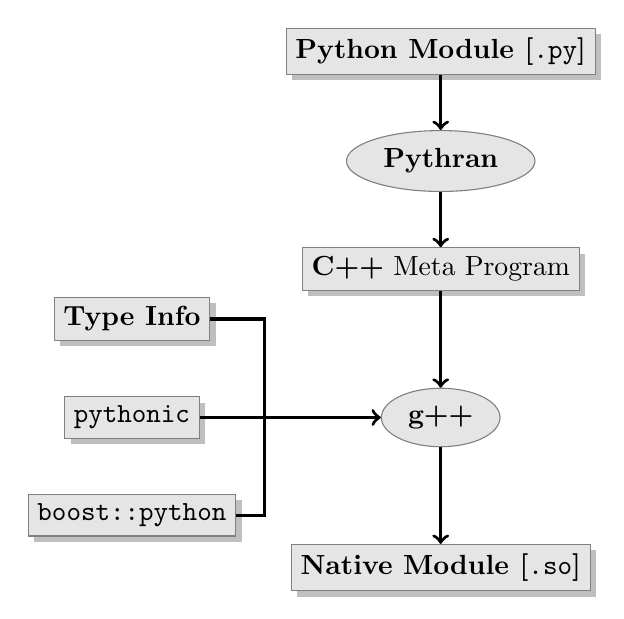
\begin{tikzpicture}[
            file/.style={draw=black!50,fill=black!10,rectangle, drop shadow, align=center,
            node distance=0.7cm},
            tool/.style={draw=black!50,fill=black!10,ellipse, align=center, node
        distance=0.7cm}]
        \node[file] (python) {\textbf{Python Module [\texttt{.py}]}};
        \node[tool] (pythran) [below=of python] {\textbf{Pythran}};
        \node[file] (meta-cxx) [below=of pythran] {\textbf{C++} Meta Program};
        \node[tool] (gxx) [yshift=-1.5em, below=of meta-cxx] {\textbf{g++}};
        \node (empty) [xshift=-1em, left=of gxx] {};
        \node[file] (pythonic) [left=of empty] {\textbf{\texttt{pythonic}}};
        \node[file] (annotation)     [above=of pythonic] {\textbf{Type Info}};
        \node[file] (boost) [below=of pythonic] {\textbf{\texttt{boost::python}}};
        \node[file] (so) [yshift=-1.5em, below=of gxx] {\textbf{Native Module [\texttt{.so}]}};

        \draw[very thick, ->] (python) -- (pythran);
        \draw[very thick] (annotation) -| (empty.center);
        \draw[very thick, ->] (pythran) -- (meta-cxx);
        \draw[very thick, ->] (meta-cxx) -- (gxx);
        \draw[very thick] (boost) -| (empty.center);
        \draw[very thick, ->] (pythonic) -- (gxx);
        \draw[very thick, ->] (gxx) -- (so);
    \end{tikzpicture}

    \caption{Pythran compilation flow.}
    \label{fig:pythran-compiler}

\end{figure}


\subsection{Expermimental Setup}

\subsection{Results and Analysis}

%%
%%
\section*{Conclusion}

\acks

The Pythran project is an independent Open Source initiative that has been
partially funded by the CARP Project and the SILKAN Company.

Several Students of Télécom Bretagne, namely Adrien Merlini, Alan Raynaud,
Xavier Corbillon, Yuancheng Peng and Eliott Coyacc, have made significant
contributions to the project.

% We recommend abbrvnat bibliography style.

\bibliographystyle{abbrvnat}
\bibliography{biblio}


\end{document}
